\chapter{Formalizing Scheme}
Any proof about properties of Scheme, such as a proof about semantic preservation over a transformation, needs to be based on a formal definition of the language. Therefore, our first step in writing such a proof is to formally define the Scheme language. For the sake of simplifying the proof, we excluded many features --- in general, these are features where our transformation doesn't change very much, but are complex enough to add substantial difficulty to our proof. These excluded features are discussed in more detail in section \ref{sxn:excluded}.
\section{R6RS Scheme}
Fortunately, Scheme is already well-defined. The R6RS language standard \cite{sperber_revised6_2009} provides a formal specification of Scheme's syntax and semantics, and also gives an implementation of the semantic model in the PLT Redex language. As previously mentioned, we excluded many features from this formal definition for ease of reasoning. Below is our modified version of R6RS Scheme

\subsection{Syntax}
Figure \ref{fig:syntax} shows an EBNF representation of the syntax for our subset of Scheme.
\newpage
\begin{figure}[h]
    \centering
\begin{bnfgrammar}
    P ::=
        (store (sf ...) e)
    ;;
    sf ::=
        (x v)
    |   (pp (cons v v))
    ;;
    e ::=
        nonproc
    |   proc
    |   (begin e e ...)
    |   (if e e e)
    |   (e e ...)
    |   (set! x e)
    |   (values v)
    |   x
    ;;
    v ::=
        nonproc
    |   proc
    ;;
    nonproc ::=
        pp
    |   null
    |   n
    |   \#t
    |   \#f
    ;;
    proc ::=
        (lambda (x) e)
    |   (lambda () e)
    |   car
    |   cdr
    |   cons
    |   set-car!
    |   set-cdr!
    |   +   
    |   -
    |   /
    |   *
    ;;
    pp ::=
        [pair pointers]
    ;;
    x ::=
        [variables]
    ;;
    n ::=
        [integers]
\end{bnfgrammar}
\caption{The syntax for our subset of Scheme}
    \label{fig:syntax}
\end{figure}

Variables and pair pointer names are restricted to exclude keywords.

\subsubsection{Evaluation Contexts}
While we have presented a syntax for programs in our language, as we will see in the next section, our semantics operates on programs decomposed into an \textit{evaluation context} and a reducible expression.

Evaluation contexts utilize a syntax of \textit{holes} and \textit{contexts} to isolate certain sub-expressions in order to apply semantic rules on them.

For example, we can decompose the following program to allow for evaluation of the expression in the \textit{$e_1$} position of the if expression.

$(store\ (sf\ \dots)\ (if\ ((lambda\ (x)\ \#t)\ 5)\ \#t\ \#f)) = C[((lambda\ (x)\ \#t)\ 5)]$ where $C = (store\ (sf\ \dots)\ (if\ [\ ]\ \#t\ \#f)$.

The key feature of evaluation contexts is that they can control where evaluation occurs. These contexts cleverly enforce a canonical order of evaluation. In our case, since we restrict the R6RS semantics such that any expression that is reducible has only one possible step to take, this means that our semantics is deterministic. We prove this property of our semantics in section \ref{sxn:det_sem}.

Since we have removed many features, we use only the evaluation contexts relevant to expressions that are still in our language:

\begin{figure}[h]
    \centering
\begin{bnfgrammar}
    C ::= (store (sf ...) $F_{*}$)
    ;;
    F ::= [ ]
    |   (v ... $F_{\circ}$ v ...)
    |   (if $F_{\circ}$ e e)
    |   (set! x $F_{\circ}$)
    |   (begin $F_{*}$ e e ...)
    ;;
    $F_{*}$ ::= [ ]$_{*}$
    |   F
    ;;
    $F_{\circ}$ ::= [ ]$_{\circ}$
    |   F
\end{bnfgrammar}
    \caption{The evaluation contexts for our subset of Scheme}
    \label{fig:eval_ctx}
\end{figure}

Here, $F_{*}$ and $F_{\circ}$ refer to contexts that perform promotion or demotion between single values and (values v) expressions. The relevant semantics rules are presented in figure \ref{fig:Sem2}. Though we do not support multiple values, we wanted to preserve this feature of the formal semantics to increase extensibility of our subset, as well as ensure that our semantics is a true subset of the R6RS semantics. It also means that our proofs will be more easily adaptable if the language is modified to include multiple values.

\subsection{Semantics}
Figures \ref{fig:Sem1} and \ref{fig:Sem2} show the operational semantics for our subset of Scheme.
\begin{figure}
\centering
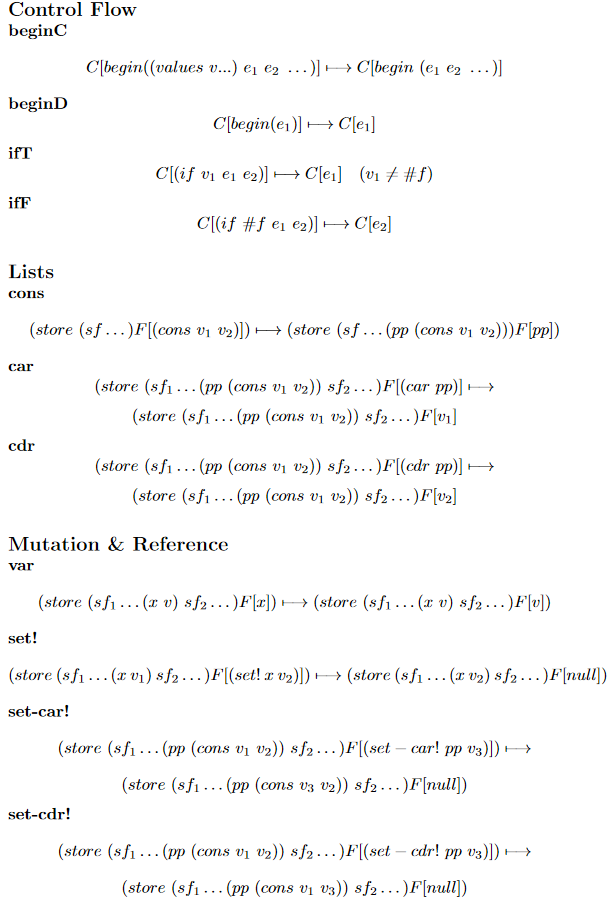
\includegraphics[width=\textwidth,height=\textheight,keepaspectratio]{figures/sem_1.png}
    \caption{Control flow, list, and mutation semantics for our subset of Scheme}
    \label{fig:Sem1}
\end{figure}

\begin{figure}
\centering
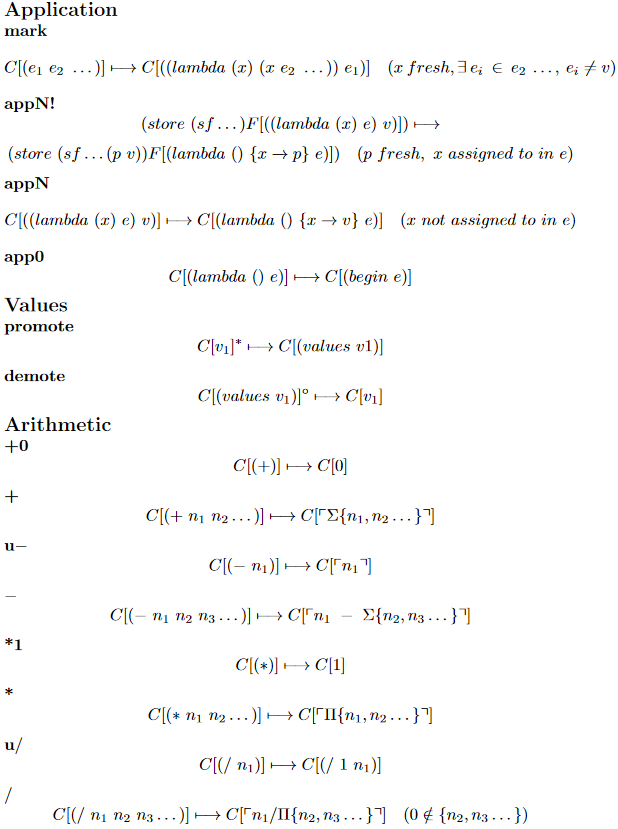
\includegraphics[width=\textwidth,height=\textheight,keepaspectratio]{figures/sem_2.png}
    \caption{Application, value handling, and arithmetic semantics for our subset of Scheme}
    \label{fig:Sem2}
\end{figure}

We define x being "assigned to" as x being the target of a set! expression.

Some discussion of our semantic rules and how they work together to evaluate Scheme programs is required.

\subsubsection{Control Flow}\label{sxn:sem_cf}
\textbf{beginC} works by removing values from the front of a $(begin\ \dots)$ expression. Together with the begin evalaution context, \textbf{beginC} evaluates and removes each sub-expression in a $(begin\ \dots)$ expression until it has only a single sub-expression remaining. Then, the \textbf{beginD} rule applies to consider that expression alone. This is how the requirement that Scheme begin expressions return the value of the last sub-expression is enforced.

\textbf{ifT} and \textbf{ifF} behave as expected, with the minor quirk that any value that is not $\#f$ is considered true.

\subsubsection{Lists}\label{sxn:sem_lists}
\textbf{cons}, \textbf{car}, and \textbf{cdr} handle pairs (and therefore lists) in our language. Notably, \textbf{cons} places pairs into the store and returns a pointer to the store location in return. \textbf{car} and \textbf{cdr} therefore take a pair pointer as their argument to access the first and second values of the pair respectively.

\subsubsection{Mutation \& Reference}\label{sxn:sem_assign}
\textbf{var}, \textbf{set!}, \textbf{set-car!}, and \textbf{set-cdr!} handle assignment in the language. \textbf{var} is a fairly straightforward step that takes a variable referring to a store location and returns the value at that location. The assignment functions replace values in a store location in a similar way. One thing to note is that \textbf{set!} requires that its variable argument already exists in the store. As we are not considering top-level variables (see section \ref{sxn:excluded}), \textbf{set!} can only modify existing store locations created during lambda application.

\subsubsection{Application}\label{sxn:sem_app}
\textbf{mark} isolates un-evaluated sub-expressions from an application. By lifting an expression into a single application, either the \textbf{appN} or \textbf{appN!} Note that \textbf{mark} enforces a left to right evaluation order.

\textbf{appN!} is the application semantic rule for lambda expressions that contain assignment in their bodies. Since naive assignment into such lambda expressions would result in erroneous expressions like (set! 4 5), \textbf{appN!} first creates a fresh store location containing the value to be substituted and then performs substitution with a pointer to that location rather than with the value itself. Then, assignments inside the lambda expression's body can properly evaluate. The \textbf{appN} rule applies naive substitution in lambda expressions that do not contain assignment. As we will see in section \ref{sxn:ca-pass}, excluding these non-assigned variables from the store is integral to our proof of correctness of the compiler pass we are considering.

\subsubsection{Values \& Arithmetic}\label{sxn:sem_vals_math}
Finally the \textbf{promote} and \textbf{demote} rules deal with wrapping values to satisfy the requirements of their evaluation contexts. While this feature is vestigial in our semantics, we include it for purposes of extensibility.

The following rules present a fairly typical system for performing integer arithmetic. Note the side conditions for ensuring no division by zero takes place.

\subsubsection{Excluded Features\label{sxn:excluded}}
In the interest of shortening a potentially extensive proof, we chose to remove many features from the formal R6RS semantics. Additionally, some features of Scheme were not originally included in the formal R6RS semantics, likely due to complexity of formalization.

The features we chose to exclude were: quote, multiple argument lambda expressions (and generally multiple values as arguments), exceptions, equivalence testing, call/cc and dynamic wind, and letrec. I/O, the macro system, and the numerical tower were originally excluded from the R6RS semantics. While this list certainly contains major features of Scheme, we believe we have captured enough of the language to accurately represent and prove correctness of our transformation.

Another quirk of the formal R6RS semantics is that evaluation order of expressions is left up to the implementation. However, this means that without modification, the semantics are non-deterministic --- application of their version of the \textbf{mark} rule results in a set of steps each representing a different choice of evaluation order. In our semantics, we modify \textbf{mark} to follow a left-to-right evaluation order. This simplification allows us to prove semantic determinism, which we use in our proof. While our transformation shouldn't be affected by a different evaluation order, it is theoretically possible that an implementation of Scheme could enforce an evaluation order that would invalidate our results. 
Finally, while set! expressions that mutate top-level variables are present in Scheme, these top-level set! expressions are converted to "set-top-level!" expressions in a pass prior to the one we are considering. Therefore, we can assume that all set! terms we encounter refer to variables in their local scope. Further, handling top-level variables in general turned out to be a major difficulty in modeling this pass. Since top-level variables are not affected by this pass, we are not including them in our subset. Therefore, we do not include letrec, as this is how top-level variables are implemented by the semantics.
